\chapter{Introduction and State of the Art}
\label{c-intro}

\section{Neuroscience, neurons and their dynamics}
% \textit{What are neurons, its dynamics and what are the To-Dos}
Neuroscience is a wide and challenging field in science. It faces crucial questions, such as the study of the neural mechanisms underlying brain activity, how can those mechanisms outcome as human cognition or behavior, how is the information processed and transferred through neural activity, how are neural diseases generated and how can we detect and treat them. 
These questions and many more have been open problems that have intrigued scientific community since the first steps on the field. Neuroscience was born as a discipline from anatomy, physiology, biochemistry and biophysics. As a broad field, it is approached from distinct perspectives and it is usually referred to by its subfields, e.g. Neurobiology, Neuropharmacology, Clinical Neuroscience, Developmental Neuroscience, Systems Neuroscience, Cognitive Neuroscience, Computational Neuroscience, Neurotechnology, etc. All these fields aim to explain or repair the brain function either as a whole or in parts. They use different techniques and approaches where some of which give rise to entirely new fields, like Neuroimaging.

We cannot think or discuss about neuroscience without highlighting the work by Santiago Ramón y Cajal, crucial in the firsts steps on the understanding the brain  \parencite{ramon_y_cajal_textura_1899,de_carlos_historical_2007,de_castro_editorial_2016,delgado-garcia_cajal_2015,de_castro_cajal_2019}. The idea of the "neuron doctrine" was a boost on the study of the brain, explaining and describing the structure of individual cells called \textit{neurons} that are able to connect and thus communicate by \textit{synapses}. Figure \ref{cajal-neuron} shows one of Cajal's drawings describing a cerebellar circuit.

\begin{figure}[htb!]
    \centering
    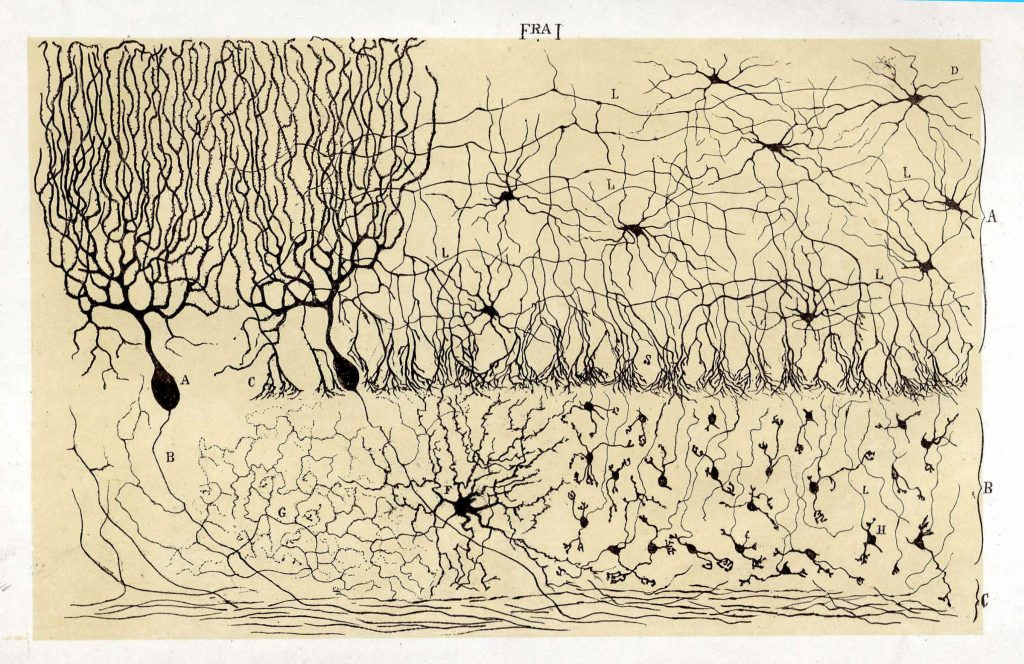
\includegraphics[width=\textwidth]{img/intro/CajalCerebellum.jpeg}
    % https://es.wikipedia.org/wiki/Doctrina_de_la_neurona#/media/Archivo:CajalCerebellum.jpg
    % https://microbioblog.es/la-fascinante-historia-de-la-reazione-nera
    \caption{Representation of cerebellar neurons by Ramon y Cajal.}
    \label{cajal-neuron}
\end{figure}

%From that starting point there have been important findings in the neurons types and structures, such as Glia cells \ref{}. 

The brain is a complex system that we can study from many different prisms. In this thesis, we follow a bottom-up approach. So we will analyze experimentally and theoretically the neural activity at ionic channels and small circuits (with few synapses). Moreover, we will follow a Neurocomputational perspective based on hierarchical sequential information processing, which will be defined in detail in subsection \ref{sec:computational neuroscience}. In the following lines we will approach the basis of neural activation from a computational perspective necessary for the reading flow of this document. We will focus not in their molecular properties but in the change of voltage that they are able to produce and how that inter-operates to give rise to neural activity. 

\subsection{Neuronal dynamics}
Neurons are cells morphologically composed by dendrites, where the connections from other neurons are received through synapses), a soma or cellular body (where information in typically integrated) and an axon (where the information is conveyed as output). Since neurons are the cells that present the largest diversity in morphology, this description does not apply to all neuronal types but serves to start highlighting the importance of spatial scales in the nervous system. 

% As said there are many different ways to study neural dynamics, but a common descriptor for neural activity are action potentials. Action potentials are the 
Neuronal electrical activity is often described in terms of the evolution of membrane voltage caused by the flow of ionic channels between the inside and outside of the cell \parencite{kandel_principles_2012}. The characteristic fast change in the membrane voltage when a neuron fires an output signal is called an action potential or a spike. They are often seen as the minimal pieces of information for reception, processing and transmission carried out by neurons. A more concrete definition of spike could be "an abrupt and transient change of membrane voltage that propagates to other neurons via a long protrusion called an axon" \parencite{izhikevich_dynamical_2007}. Thus, when no inputs are received, the membrane potential of a neuron is negative and it is called resting potential. When this potential is altered by an input that makes the voltage increase, it is known as depolarization. After reaching a peak of voltage, typically a positive value of around 40mV, the potential starts decreasing again. When the potential is more negative than the resting potential, it is known as hyperpolarization. Figure \ref{fig:action potential} illustrates the sequential phases of the action potential generation. 

\begin{figure}[htb!]
    \centering
    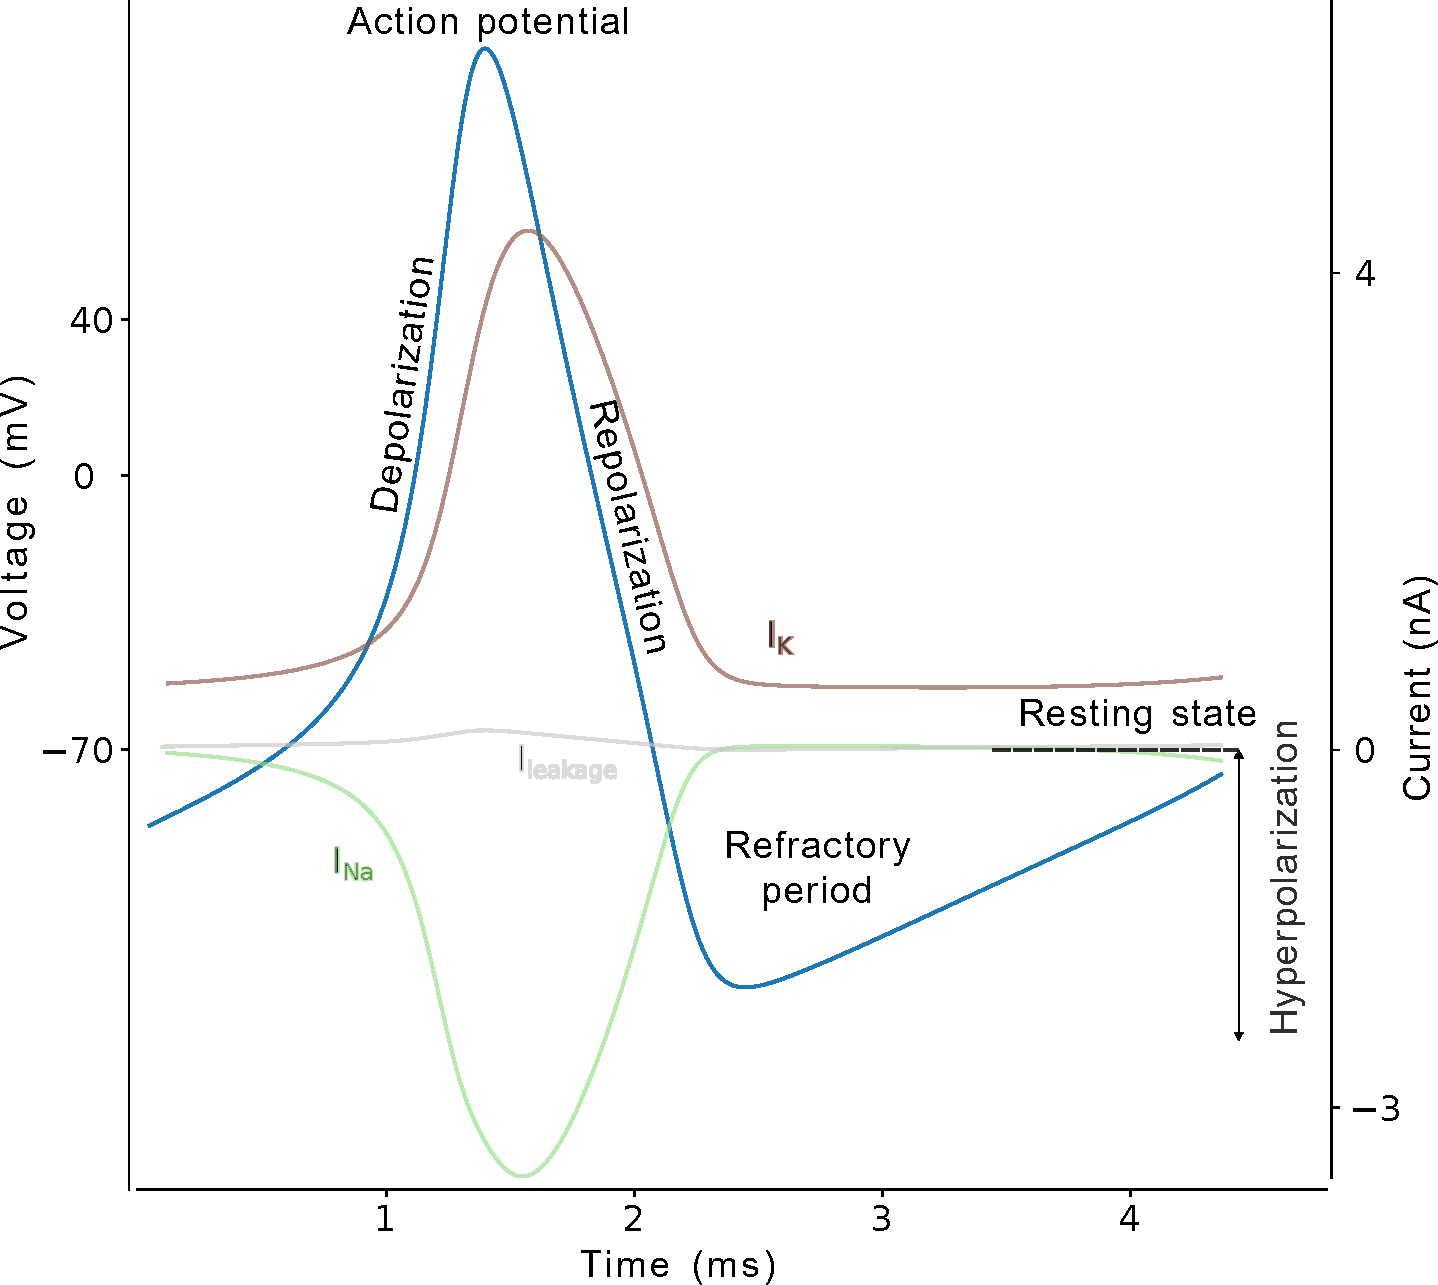
\includegraphics[width=0.8\textwidth]{img/intro/action_potential.pdf}
    \caption{Representation of the sequential  phases and terminology of an action potential. (Adapted from Chris73, Wikimedia Commons, \href{https://creativecommons.org/licenses/by-sa/3.0/}{CC BY-SA 3.0}). In each of this phases of the action potential generation, different ionic channels are activated sequentially, e.g. the sodium channel is involved during the depolarization phase and its activity decais as the potassium channel activates mostly in the repolarization phase. }
    \label{fig:action potential}
\end{figure}

The neural activity is generated by the flow of different ionic channels that counterbalance the voltage value generating the action potential \parencite{koch_biophysics_1999}. The membrane can be composed by different ionic channels, and their dynamics are conditioned by that combination and the possible synaptic connections. These changes in dynamics can be manifested in different ways, but the most notorious ones are the shape and temporal evolution of the action potential. %p61 The Neuron 
For example, in Fig. \ref{fig:spike-types} there is an example of two distinct action potentials with visible differences in their shape, one of them presents a symmetrical shape, where depolarization and repolarization slopes are similar, whereas in the right waveform, there is a notable shoulder in the repolarization and its timescale is almost double in comparison of the example shown in (a).

\begin{figure}[htb!]
    \centering
    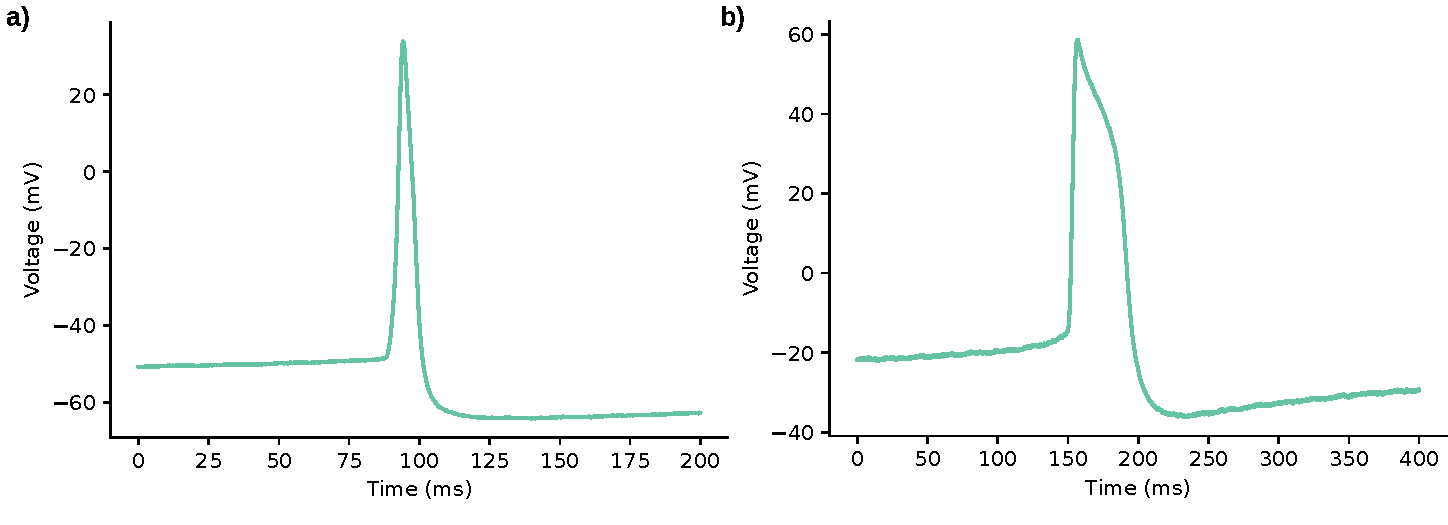
\includegraphics[width=\linewidth]{img/intro/spike-types.pdf}
    \caption{Examples of different spike shapes. Representation of two recordings from two different cells in the right parietal ganglion of \textit{Lymnaea stagnalis}. Left: symmetrical spike; right: shoulder shaped spike.}
    \label{fig:spike-types}
\end{figure}

If spikes are considered minimal pieces of information when coding the neural activity, the combination of these minimal information leads to new forms of information, also known as bursts. Although there is not a fixed description of a burst, and depending on the animal and system a burst might look different \parencite{russell_bursting_1978,palmu_detection_2010,lundqvist_gamma_2016}, there are some common features in bursts: they typically consists of a group of spikes(more than two) on top of a sustained depolarization, and these groups are separated by a hyperpolarization quiescent period called inter-burst interval (IBI). Figure \ref{fig:spike_activity-types} shows several examples of distinct neuronal activities observed in intracellular recordings. Depending on the specific neuron and the circuit, neurons can present tonic firing (first column), at different rates, or bursting activity (second column). 
\begin{figure}[htb!]
    \centering
    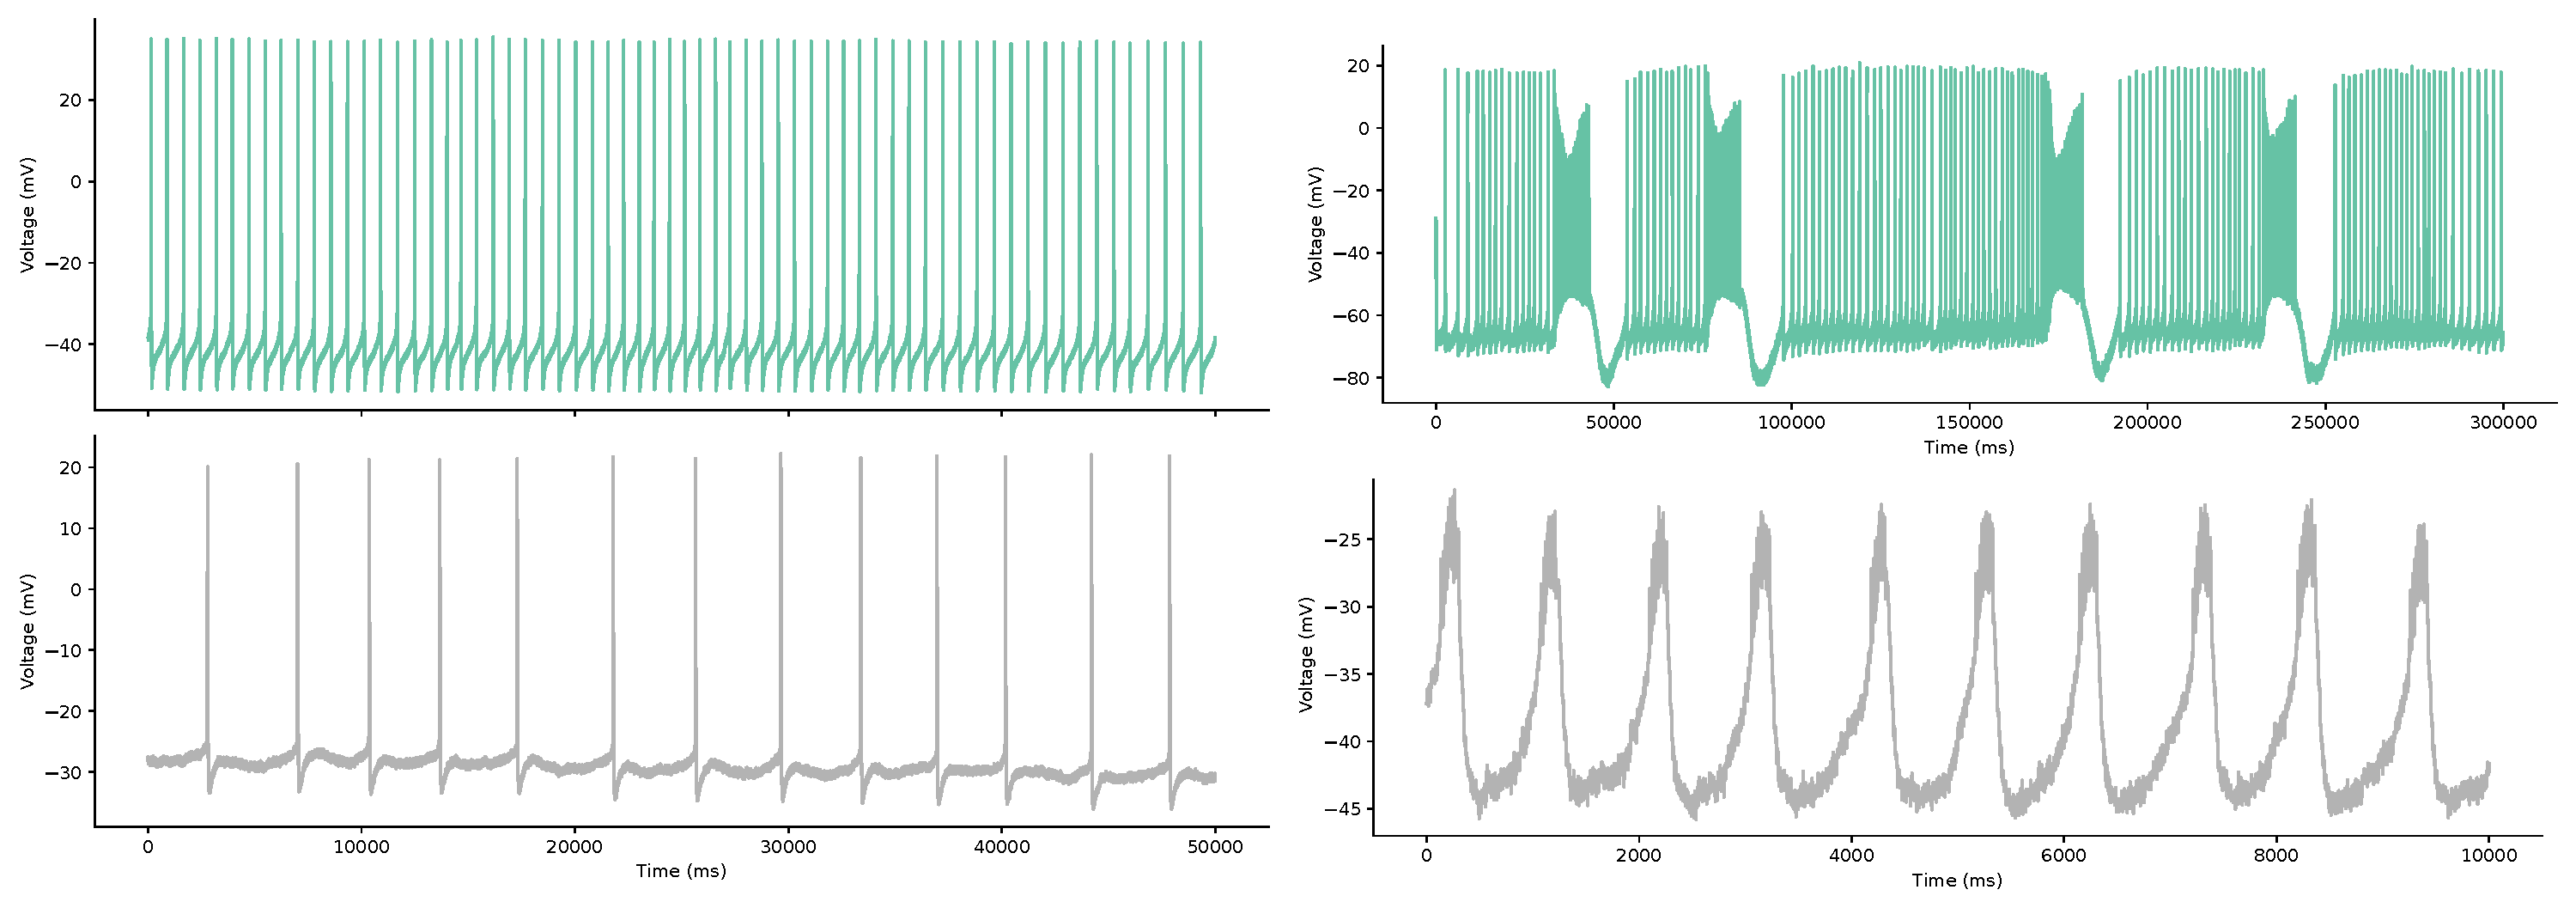
\includegraphics[width=\linewidth]{img/intro/spike_activity-types.pdf}
    \caption{Representation of two examples of different spiking neuronal activity. Left: two simultaneous intracellular recordings in \textit{Lymnaea stagnalis} showing tonic firing at two different frequencies. Right: Two examples of bursting activity, from \textit{Lymnaea stagnalis} (top panel) and from \textit{Carcinus maenas (bottom panel).}}
    \label{fig:spike_activity-types}
\end{figure}

Traditionally, neural codes have been studied focusing on the single spike activation, e.g., by the binarization of the activity (the neuron generates a spike or it does not). Burst can also be informative in terms of the neural activity, either as a whole piece of information or as a complex box of data itself: "bursts are a family of firing patterns that trigger physiological mechanisms not engaged by the same number of spikes in relative isolation" \parencite{friedenberger_silences_2023}. Bursts can be originated either by internal activation, mostly by calcium channels or by the synaptic dynamics involving the corresponding cell (inhibition/excitation) (for an extended review see \parencite{friedenberger_silences_2023}). This is the case in many Central Pattern Generators (CPGs) \parencite{Katz,steuer_central_2018}, which will be discussed in detail bellow and in Chapter \ref{c-invariants-model}.

\subsection{Network dynamics}

Although analyzing the activity of a single neuron is important in terms of characterizing its dynamics, when talking about information processing and behavior, it is also crucial to study the overall circuit dynamics. A circuit of neurons is defined by nervous cells interconnected by synapses. There are two main types of synapses in the nervous system: electrical and chemical connections, see Fig. \ref{fig:synapse-types}. The main difference between them relies on how the communication takes place. Chemical synapses occur through the mediation of \textit{neurotransmitters}, where a presynaptic neuron liberates these molecules that are bound to neuroreceptors to produce an alteration in the postsynaptic neuron. Thus, this connection is asymmetrical and unidirectional, whereas in electrical synapses we find a symmetrical and bidirectional connection. In those synapses, the neurons are almost attached by a structure called \textit{gap junction}, which "pipes" both neurons, in a tissued structure that constrains the leakage to the extracellular space. This communication allows electric charge to flow from one neuron to the other and is then faster than the chemical synapses, which in comparison has no delay. The activity of neurons electrically coupled is usually synchronous \parencite{levitan_neuron_2002}.

\begin{figure}[hbt!]
    \centering
    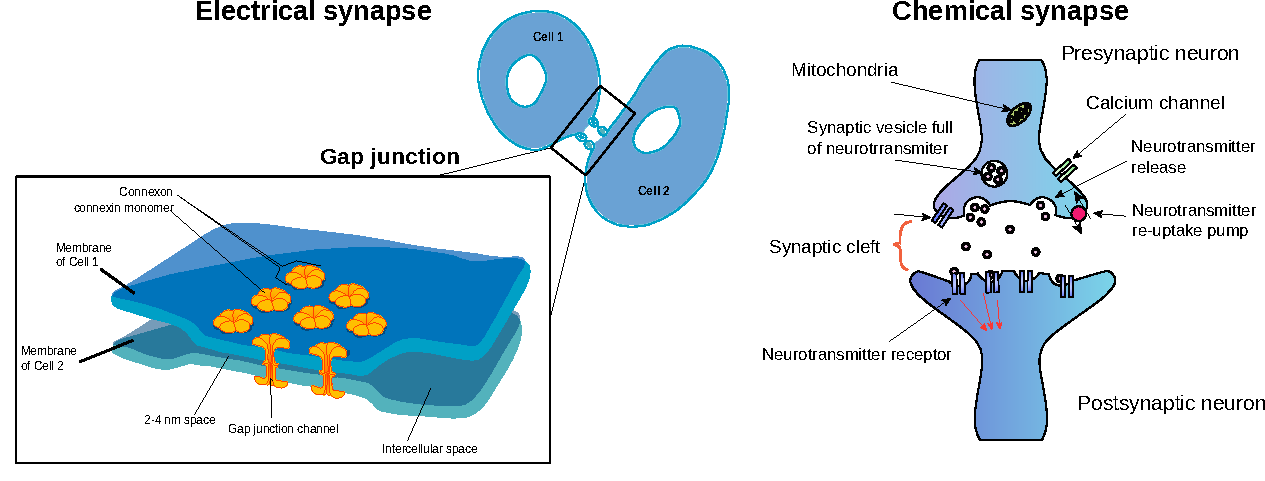
\includegraphics[width=\linewidth]{img/intro/synapses.pdf}
    \caption{Representation of synapses types. Left. Example of electrical synapse between two cells and diagram of gap junction (Adapted from \href{https://commons.wikimedia.org/wiki/File:Gap_cell_junction-en.svg}{Wikimedia Commons}). Right. Example of chemical synapse structure (Adapted from \href{https://commons.wikimedia.org/wiki/File:Synapse_diag1.svg}{Wikimedia Commons})}
    \label{fig:synapse-types}
\end{figure}

In neural circuits, cells  can be connected by one or both types of chemical and electrical synapses, and they usually are also connected to other circuits or modulatory neurons. In Figure \ref{fig:neural circuits} illustrates two examples of circuits at the cellular and macroscopic levels. In this context, there are formed complex system of networks of networks, that might work at different time scales and can take part in one or several functionalities. This interconnection of networks and, from a lower level, cells, leads to sequential activations and transfers of actions into sequences of sequences.

%% Se puede comentar que todas las redes en un circuito neuronal forman parte de otras redes como subcircuitos, que en muchos casos son multifuncionales y que redes de redes generan secuencias de secuencias en lo que se refiere a neural activations

\begin{figure}[hbt!]
    \centering
    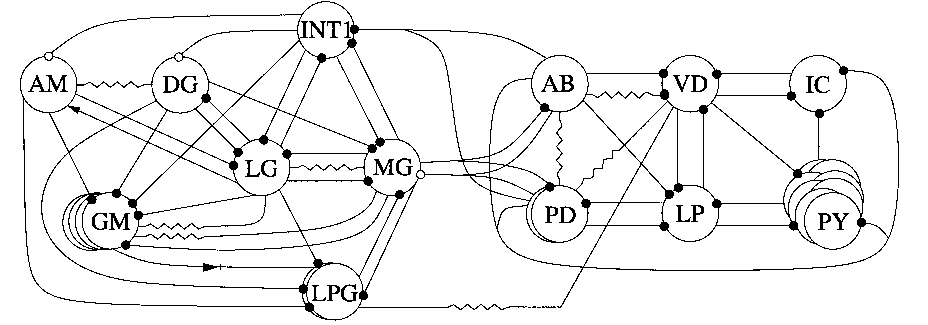
\includegraphics[width=0.64\textwidth]{img/intro/cpg diagram.png}
    \includegraphics[width=0.35\textwidth]{img/intro/The_Human_Connectome.png}
    \caption{Left. gastric and pyloric circuit scheme of \textit{Carcinus Maenas} \parencite{huerta_topology_2001}. Right. Conectome in human brain rendered from 20 subjects (By Andreashorn - Own work,\href{https://commons.wikimedia.org/w/index.php?curid=41581320}{CC BY-SA 4.0})}
    \label{fig:neural circuits}
\end{figure}

\section{The sequential nature of neural dynamics}
%the complex landscape of unanswered questions in the field of neuroscience, from a bottom-up approach.
Brain dynamics can be described as sequences of interactions, from molecules, to neurons, to motor movement and behavior, within a coordinated hierarchy of temporal and spatial scales \parencite{kiebel_hierarchy_2008,yuste05,rabinovich_discrete_2018,Rabinovich23},  from ionic channel activations to sensory encoding, processing, and decision making. Its study reveals fundamental aspects of brain function and cognition, e.g., impulse transmission, executive function, spatial processing or memory.

% There are many important cognitive processes that rely in sequential processes such as perception, memory, decision making, attention and emotion. %Binding \parencite{Michel and coegin 2018, Ravinovich 2020, He 2018}.
% Sequentiallity involves complex pieces of dynamical activity, that when incapsulated as units, can be seen as a chain of events with sequential behaviour \parencite{Ravinovich,2023}.


% Sequential activvation for unsuppervised learning/activity.

%Principles of Brain Dynamics: Global State Interaction Book
%https://www.frontiersin.org/articles/10.3389/fnsys.2014.00219/full
%https://www.ncbi.nlm.nih.gov/pmc/articles/PMC8367843/


%Kiebel 2009
%"Dynamic sequences are generated on various time-scales"
%"Brain is a recognition system that uses an internal model of its environment"

%Kiebel 2008
%"Many aspects of brain function can be understood in terms of a hierarchy of temporal scales at which representations of the environment evolve"


 A common example of sequential  processing is speech, where sequential patterns are present in the structure of phrases, as a sequences of sequences of syllables, words and silences \parencite{kiebel_recognizing_2009}. In this line, an extended case of study is the birdsong, which has  similarity to human's speech, as they involve sequences of coordinated sounds \parencite{prather_brains_2017,fishbein_sound_2019}. Beyond speech, sequential processing is also present in motor movement, from muscle activation to repetitive coordinated actions such as rhythmic tapping or music performance \parencite{ding_temporal_2017}. Also, there are many important cognitive processes that rely in sequential mechanisms such as perception, memory, decision making, attention and emotion \parencite{Varona2016, he_robust_2018, rabinovich_sequential_2020}.

However, it is not clear how exactly the brain processes time. In contrast to the theory of a central clock that manages time for every behavioral task, the theory of a distributed time processing \parencite{buonomano_temporal_1995,ivry_representation_1996} is well accepted. In this framework, especially in movement coordination, there is a need for circuits that manage the sequential rhythmic activity. This is the case of Central Pattern Generators (CPGs), circuits of neurons with closed-topology that sequentially activate neurons and generate coordinated motor activity \parencite{selverston_reliable_2000}. They are present in many systems, from insects to humans \parencite{pearson_central_1972,marder_central_2001,mackay-lyons_central_2002,minassian_human_2017}. There are several key aspects that make these circuits an interesting case of study. First, their neurons are organized in closed-topologies receiving all feedback from companion cells \parencite{huerta_topology_2001}. These circuits are able to maintain a rhythmic activity in an autonomous manner, typically by mutual inhibitory interactions~\parencite{katz_evolution_nodate}. Second, their activity is flexible enough to adapt to changes in the context, e.g., variations in the terrain while walking. Finally, they are present in many systems and in some of them there is a direct relationship between the activity of the neurons in the circuit and the motor movement that they produce. For example, in the stomatogastric CPG in the crab \textit{C. maenas}, in charge of the pylorus movement, the PD (pyloric dilator), LP (Lateral Pyloric) and PY (PYloric) neurons correspond to the pylorus dilatation, pylorus close and contraction of the rostral constrictor to move food in the digestive system \parencite{moulins_introduction_1987,selverston_oscillations_2006}.

\begin{figure}[hbt!]
	\centering
	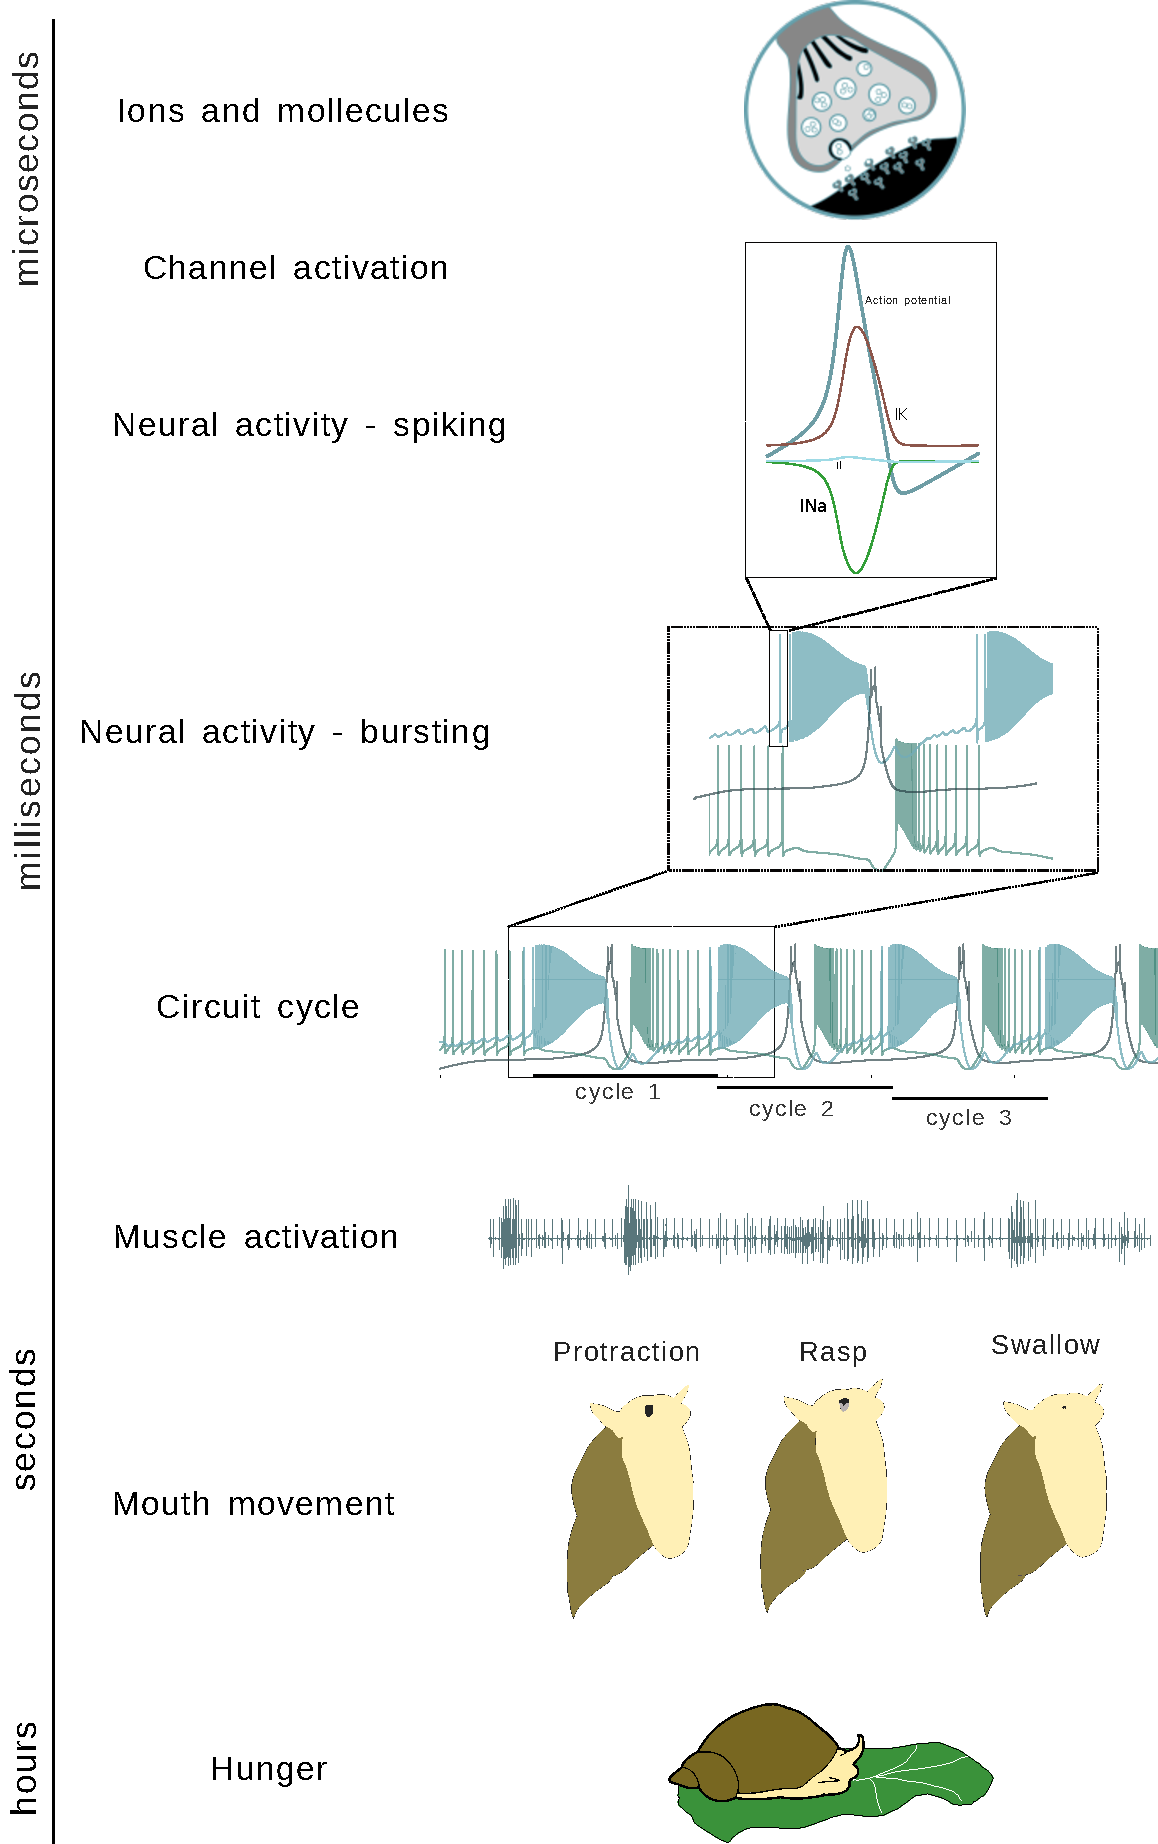
\includegraphics[width=0.9\textwidth]{img/intro/time scale/time-scale-feeding.pdf}
	\caption{Illustration of the sequential feeding process at different time scales in {\sl Lymnaea stagnalis}.}
	\label{fig:time scale feeding}
\end{figure}

The sequential activity in the brain goes from the sub-millisecond scale to days (the time scale of circadian rhythms \parencite{mauk_neural_2004}). Figure \ref{fig:time scale feeding} shows an illustrative example of the sequential nature of neural activity at different scales in the generation of coordinated motor activity in the feeding of a snail. At the scale sub-milliseconds, there is a flow of ions that generate a sequence of ionic channel activation, that in the scale of milliseconds produce action potentials. The combination of them in form of rhythmic bursts, activate the corresponding muscles at the scale of seconds and generate the necessary sequential movement to eat: open the mouth, rasp food and swallow, that is  repeated along the day. 


The study of the action potential dynamics and the interaction between ionic channels and synapses is crucial, since it is a key part in any brain process, and it cannot be detached from the whole. The alteration of the dynamics of these channels at different sites along the neuron can affect synaptic inputs/outputs, how the neurons communicate and the resulting process. Ionic channels are the starting point of the electrical signals underlying neuronal network activity, and their malfunction can contribute to neural disorders \parencite{kecskes_editorial_2023}. Thus, understanding brain activity not only at large scales but also from the stage of voltage generation dynamics can be crucial for a real and complete understanding of neural systems. Their study can also help distinguish between short- and long-term modulation, a key aspect in neural plasticity and the application of neuromodulatory techniques \parencite{chambers_light-activated_2008,burke_modulation_2019}.

%Regarding sequential studies, it is common to talk about neural activity as blocks of information and as a binary on-off event, even for whole brain areas, classifying tasks by those findings. Although the findings under this approach have been undoubtedly relevant, they usually do not consider the importance of dynamics, variability and how their processing affects behavior.
 
%Although often disregarded in macroscopic studies and as a consequence in bottom-up approaches,
It is important to explore the mechanisms that allow to maintain a robust sequential activity despite changes in context and the variability underlying the neural dynamics. Action potentials and bursts can be classified depending on their waveform shape and grouped spiking activity. However, in those subgroups there is a high intra-variability, where for example bursting activity can differ in shape and duration, i.e., number of spikes in a bursts. Figure \ref{fig:burst variability} shows an example of the variability in the burst waveform and duration for a sequence of several bursts. 


\begin{figure}[htb!]
	\centering
	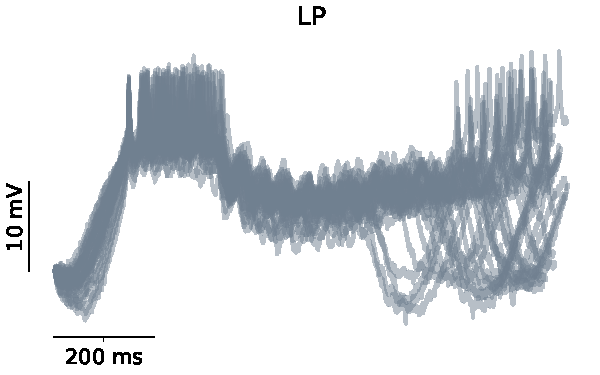
\includegraphics[width=0.6\textwidth]{img/intro/burst_variability.pdf}
	\caption{Superimposition of bursts at different time instants aligned by the first spike in the burst for intracellular recordings of an LP neuron in the sthomatogastric CPG.}
	\label{fig:burst variability}
\end{figure}

The study of this variability unveils key factors in the sequentiallity and how it is maintained despite different intrinsic or external modulations. This is the case for example of sequential dynamical invariants, i.e., robust relationships between time intervals that conform a neural sequence, when analyzing the activity cycle-by-cycle \parencite{reyes_artificial_2008,elices_robust_2019,garrido-pena_characterization_2021,berbel_emergence_2024}. This sequential dynamical invariants might have a crucial role understanding the coordination of sequential activity and the balance between robustness and flexibility required for effective function in many brain processes \parencite{tatsuno_analysis_2015,ullen_neural_2003,zimnik_independent_2021,zhou_neural_2020,dragoi_cell_2020}. We will discuss in detail this phenomena in the feeding CPG of \textit{Lymnaea stagnalis} in chapter \ref{c-invariants}.


\section{Studying neural dynamics in computational models.}
\label{sec:computational neuroscience}
Computational Neuroscience is a subfield of neuroscience that uses theoretical and computational techniques to address the study of nervous system at multiple levels, from the molecular level all the way to the complex networks that shape behavior. It is thus a multi-disciplinary field. The basis of Computational Neuroscience lay on the understanding of brain dynamics from its electrical signals and the information they carry \parencite{schwiening_brief_2012,catterall_hodgkin-huxley_2012,dimitrov_information_2011,shannon_mathematical_1948}. Computational Neuroscience has extended its scope, leading to new paths of research including complex networks, graph theory, single cell analysis and machine learning techniques \parencite{cns2023}. In fields such as Artificial Intelligence there is even a symbiotic relationship between fields, where both inspire and help each other grow \parencite{amunts_human_2019,wozniak_deep_2020,goncalves_training_2020}.

An important part of Computational Neuroscience is the description of neural systems with theoretical models and the reproduction of key phenomena by the model simulation. The simulation of neural activity is a powerful tool to explore neuronal dynamics, its biophysical sources, the possible mechanisms underlying the neural signaling, and the observed complex information processing. Its strength relies on the complete accessibility to the variables of the model, the typical extensive range of tunable parameters in the model which can be explored,  and the ability to assess the role  of distinct elements in the system or circuit by including or excluding them in the simulations. Although models cannot fully substitute research on living systems, they do lead us closer to the understanding of complex neural dynamics, being a fast, effective and a low cost alternative to advances in science.  Also, models are an essential complement to experimental neuroscience reaching detailed descriptions where experimental approaches such as electrophysiology have limitations arising from the always present partial observability. 
%Like science is not about truth, but about knowledge, models do not aim to substitute living systems, but to lead us closer to the insight of neural dynamics. %#ToDo revisar

Models can be classified by their level of description, i.e. what level of simplification/abstraction is used, the detail of the structure/phenomenon being modeled and the size of the network, or their ability to reproduce the observed neural activity, e.g. chaotic dynamics. Figure \ref{fig:models-classification} illustrates such kind of classification, with examples of models of large networks as \cite{potjans_cell-type_2014,bezaire_interneuronal_2016}, of single cell but still detailed as in \cite{smith_dendritic_2013} and more abstract descriptions such as the one proposed in \cite{izhikevich_simple_2003}. Regarding the level of description, in the different biophysical models there is always a choice between detailed description of non-linearities, channels and excitation properties, and efficiency in computation. In this line, researches can choose from conductance-based models  \cite{hodgkin_quantitative_1952}, rich in the description of nonlinearities or simplified dynamical models  \cite{hindmarsh_model_1984,fitzhugh_impulses_1961}, which typically represent nonlinearities with polinomial simplifications (see \cite{torres_modeling_2012} for a review of different levels of neuronal modeling. 


%Adapt models table from
%https://www.sciencedirect.com/science/article/pii/S0896627319304441 Figure 2A:
\begin{figure}[bth!]
	\centering
	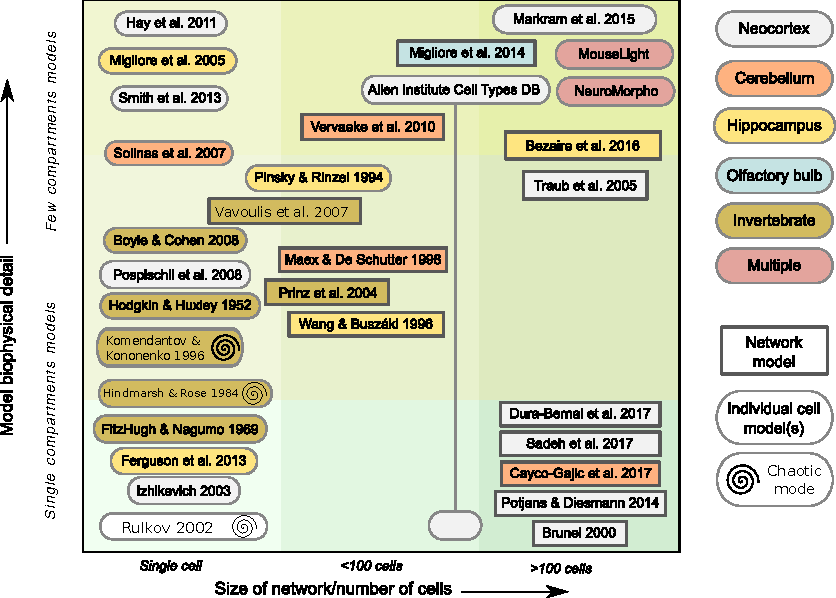
\includegraphics[width=\textwidth]{img/intro/models classification_v2.pdf}
	\caption{Neural and network models classified by biophysical detail, structure modeled and size of the network. Figure adapted from Fig. 2 \cite{gleeson_open_2019} under \href{http://creativecommons.org/licenses/by/4.0/}{Creative Commons CC-BY license}. Models are classified by the biophysical detail, by y-axes being the models in the bottom the less specific ones; by the size of the network modeled, from left to right one cell to hundreds of cells; and by the brain-structure they model, represented in colored boxes. The shape of the box also classifies the model in network model or individual cell model. A third category was here included from the original work, representing by an spiral in the box the ability of the model to produce chaotic activity without external alterations, i.e, reproduce spontaneous variability. Although the figure does not contain all model approaches, it illustrates key milestones in neuronal modeling. }
	\label{fig:models-classification}
\end{figure}
\subsection{Conductance-based models}

In this thesis, all experimental recordings have been supported with simulations on conductance-based models. They are defined as mathematical descriptions of the ionic channels dynamics, based on their voltage-dependent conductance. The pioneer study by \cite{hodgkin_quantitative_1952} defined dynamical equations based on the equivalent electrical circuit of the electrical properties of neurons in \textit{Aplysia}, see Fig.  \ref{fig:electrical circuit}. This modeled circuit is also used to conform the intracellular recording configuration, where the pipette is included as an extra current compensated by the electrode in the bath (see Fig. \ref{fig:clamp circuit}).

\begin{figure}[htb!]
	\centering
	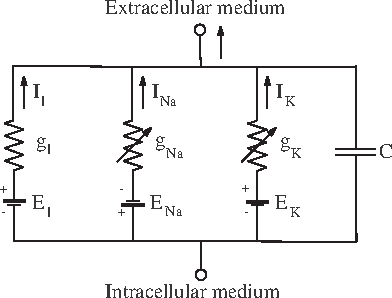
\includegraphics[width=0.7\textwidth]{./img/intro/electrical_circuit.pdf}
	\caption{Electrical circuit describing the membrane voltage in a conducatance based neuron model.}
	\label{fig:electrical circuit}
\end{figure}

\begin{figure}[htb!]
	\centering
	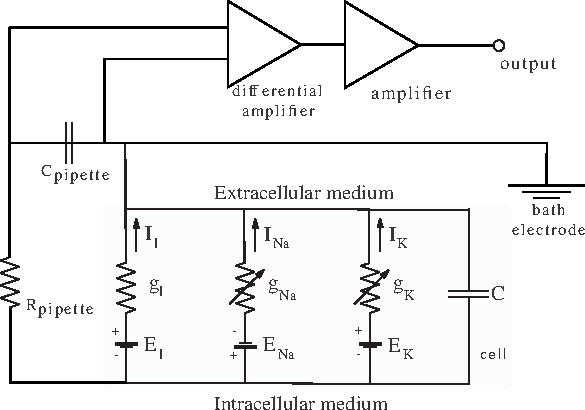
\includegraphics[width=0.7\textwidth]{./img/intro/intracellular_recording_circuit.pdf}
	\caption{Electrical circuit representing the scheme for intracellular recordings.}
	\label{fig:clamp circuit}
\end{figure}


In these models, the simulation of neural electrical activity is based on the mathematical description of different ionic channels in the circuit, whose dynamics are also well defined by activation gates. First, there is a mathematical description of the voltage dependency on time, as described by the equation \ref{eq:voltage ions}:

\begin{equation}
 C_m \frac{dV}{dt} = I - \sum I_{x},
  \label{eq:voltage ions}:
\end{equation}

where $V$ is the membrane potential, $I$ is an external current, e.g. an external stimulus or a synaptic current, $I_{x}$ is the current description for each channel involved in the action potential generation, e.g., sodium, potassium, calcium ( $I_K$, $I_{Na}$, $I_{Ca})$.

Second, each channel is also described voltage-dependent composed by activation-gates dynamics:
\begin{equation}
I_x =  g_x m^n h^n (V - E_x), 
\end{equation}

where $g_x$ is the corresponding conductance of the channel, $E_x$ is the reversal potential for that channel and $m$ and $h$ represent activation and inactivation variables, respectively.
Activation gates usually have an exponential tendency, and are defined by activation and inactivation dynamics, also dependent on voltage and time. They follow the structure in equation \ref{eq:alpha-beta}

\begin{equation}
	\label{eq:alpha-beta}
	\frac{dm}{dt} = \frac{m_{\infty,i}-m_i}{\tau_{m,i}}
\end{equation}

where $\tau_{m,i}$ are the relaxation time constants which are usually voltage-dependent and modeled using sigmoid or Gaussian functions. Note that $m$ was used here but this formula corresponds also to inactivation variables. 


Following the Hodgkin and Huxley formalism, 
the equations that describe the voltage dynamics and the conductance dynamics of the active channels (Na and K) in the circuit shown in Fig. \ref{fig:electrical circuit} are:
%\begin{equation}
%		C \frac{dV}{dt} = I - g_K n^4 (V - E_K) - g_{Na} m^3h(V-E_{Na}) - g_L (V-E_L)
%\end{equation}

% Please add the following required packages to your document preamble:
% \usepackage{multirow}
\begin{table}[h!]
	\begin{tabular}{lccc}
		Voltage equation                                                                 & \multicolumn{3}{c}{$C \frac{dV}{dt} = I - g_K n^4 (V - E_K) - g_{Na} m^3h(V-E_{Na}) - g_L (V-E_L)$}                                                                                                                                  \\ \hline
		& \multicolumn{2}{c}{Activation variables}                                                                                                                              & Inactivation variable                                        \\ \hline
		\multicolumn{1}{c|}{\begin{tabular}[c]{@{}c@{}}gating \\ variables\end{tabular}} & \multicolumn{1}{c|}{$\frac{dm(t)}{dt}=\frac{m_{\infty}(V(t))-m(t)}{\tau_m(V(t))}$} & \multicolumn{1}{c|}{$\frac{dn(t)}{dt}=\frac{n_{\infty}(V(t))-n(t)}{\tau_n(V(t))}$} & $\frac{dh(t)}{dt}=\frac{h_{\infty}(V(t))-h(t)}{\tau_h(V(t))}$ \\ \hline
	\end{tabular}
%	\begin{tabular}{cccc}
%		\multicolumn{1}{l}{Voltage equation}                                                              & \multicolumn{3}{c}{$C \frac{dV}{dt} = I - g_K n^4 (V - E_K) - g_{Na} m^3h(V-E_{Na}) - g_L (V-E_L)$}                                                                                                       \\ \hline
%		\multicolumn{1}{l}{}                                                                              & \multicolumn{2}{c}{Activation variables}                                                                                                                 & Inactivation variable                          \\ \hline
%		\multicolumn{1}{c|}{\begin{tabular}[c]{@{}c@{}}gating \\ variables\end{tabular}}                  & \multicolumn{1}{c|}{$n = \alpha_n (V)(1-n)-\beta_n(V)n$}                    & \multicolumn{1}{c|}{$m = \alpha_m (V)(1-m)-\beta_m(V)m$}                   & $h = \alpha_h (V)(1-h)-\beta_h(V)h$            \\ \hline
%		\multicolumn{1}{c|}{\multirow{2}{*}{\begin{tabular}[c]{@{}c@{}}transition \\ rates\end{tabular}}} & \multicolumn{1}{c|}{$\alpha_n(V)=0.01\frac{10-V}{\exp(\frac{10-V}{10})-1}$} & \multicolumn{1}{c|}{$\alpha_m(V)=0.1\frac{25-V}{\exp(\frac{25-V}{10})-1}$} & $\alpha_h(V)=0.07\exp\frac{-V}{20}$            \\ \cline{2-4} 
%		\multicolumn{1}{c|}{}                                                                             & \multicolumn{1}{c|}{$\beta_n(V)=0.0125\exp(\frac{-V}{80})$}                 & \multicolumn{1}{c|}{$\beta_m(V)=4\exp(\frac{-V}{18})$}                     & $\beta_h(V)=\frac{1}{\exp(\frac{30-V}{10})+1}$ \\ \hline
%	\end{tabular}
	\label{table:hh-equations}
\end{table}

This combination of channels generates the spike waveform shown in Fig. \ref{fig:spike-types model}a) but, as in living systems, the combination of different channels leads to distinct outputs, e.g. shoulder and no-shoulder type neurons (see previous section, Fig. \ref{fig:spike-types}). This is the case of waveform in Fig. \ref{fig:spike-types model} b), where this shoulder shape could be reproduced in models by including calcium specific channels.

\begin{figure}[htb!]
	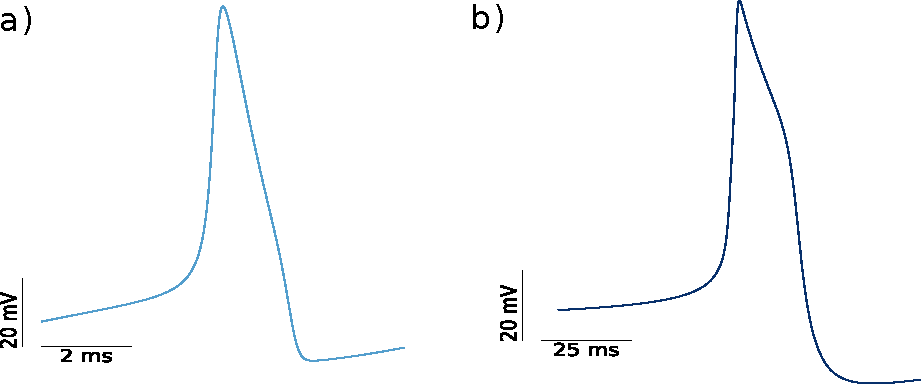
\includegraphics[width=\textwidth]{img/intro/spike-types model.pdf}
	\caption{Simulation of two distinct spike types: no shoulder (a) and shoulder shaped (b), described by equations in \cite{hodgkin_quantitative_1952} and \cite{vavoulis_balanced_2010}, respectively}
	\label{fig:spike-types model}
\end{figure}

\subsubsection{\large{Modeling networks}}
\label{c-intro-synapses}
In addition to the modeling of the action potential generation, synapses can also be modeled with different mathematical representations depending on the type and the level of specificity. Synapses are introduced in conductance-based models as an extra current that simulates the alteration in the neuron dynamics by chemical or electrical synapses. In conductance based models, electrical synapses or gap junctions are usually defined by the following equation:
\begin{equation}
    I_{ij}(t) = \bar{G}_{ij} (V_i(t) - Vj(t))
\end{equation}
\noindent where $i$ and $j$ represent the two neurons conforming the electrical synapse and $\bar{G}_{ij}$ is a constant representing the maximum value of synapse conductance in the connection. For symmetrical gap junctions, the other cells receives exactly the same current with inverse sign.

On the other hand, chemical synapses are by definition asymmetrical and can be described as in equation \ref{eq:synapse binary}:
\begin{equation}
     I_{ij}(t) = G_{ij}(t) (V_i - E_j^{syn})
     \label{eq:synapse binary}
\end{equation}
\noindent where $E_j^{syn}$ is the voltage value at which the synaptic current cancels and $G_{ij}$ can now have complex dynamics considering the trafficking of neurotransmitters as in equation \ref{eq: Gii} \parencite{torres_modeling_2012}. 

\begin{equation}
	G{ij}(t) = \bar{G_{ij}}  \Theta(t-t_j^{sp}) \alpha (t-t_j^{sp})
	\label{eq: Gii}
\end{equation}
\noindent where $\bar{G_{ij}}$ is the constant value for the conductance, ${t_j}^{sp}$ is the time at which the presynaptic spike occurs. $\Theta(x)$ is the Heaviside step function and $\alpha(t)$ is a function to model an evoked postsynaptic responses that can be defined by exponential functions.

Depending on the selection of this level of specification, the neuron can be activated by a (i) binary cause: occurrence or absence of an action potential, or (ii) a dynamic model that is also dependent on the the postsynaptic voltage level (e.g. a graded synapse) or represents phenomena such as synaptic depression or facilitation. In that second case the level of specification is higher, with a richer description of the synapse dynamics. This is the case for example of \cite{tsodyks_neural_1997}, represented in equations \ref{eq:tsodyks1},\ref{eq:tsodyks2} or the gradual synapse in the CPG model by \cite{vavoulis_dynamic_2007}, discussed in methods chapter, section \ref{sec:CPG model}.


\begin{equation}
	\frac{dU}{dt} = -\frac{U}{\tau_{\text{rec}}} + U_{\infty}(1 - U) \delta(t - t_{\text{spike}})
	\label{eq:tsodyks1}
\end{equation}
\begin{equation}
	\frac{dX}{dt} = -\frac{X}{\tau_{\text{fac}}} + (1 - X) \frac{U(t_{\text{spike}})}{U_{\infty}} \delta(t - t_{\text{spike}})
	\label{eq:tsodyks2}
\end{equation}


\subsection{Variability in computational models}

Most studies use deterministic models that produce regular neural activity, which are sufficient for many research questions when exploring input/output responses, studying the role of different biophysical elements or supporting experimental results on steady state dynamics. However, living systems are highly variable, often working in transient regimes, often displaying chaotic activity, and still able to produce sequential and robust patterned activity~\parencite{selverston_reliable_2000}. Variability in the activity of living neurons has been proven to play an important role in relevant information processing tasks. While this is a key aspect in neural dynamics, models usually exclude intrinsic variability from their description,  particularly in membrane potential waveforms and in collective adaptive dynamics. To induce some level of stochasticity, models typically include Gaussian noise as external input \parencite{linaro_accurate_2011,pezo_diffusion_2014,zheng_spontaneous_2020}. However, this is a limited approach when exploring the role of variability intrinsically and dynamically generated by the the neurons and the circuits for a specific computational tasks, e.g. for sequence coordination. There are several possibilities to include variability in neuronal intrinsic dynamics as it is the example of \cite{hindmarsh_model_1984} or \cite{komendantov_deterministic_1996}, where in both descriptions, there is a combination of parameters that lead both to a chaotic state, where the resulting activity is not regular. When the source of the variability in the system comes from its intrinsic properties, there is a possibility to study its dynamics and the role of this variability in the system without random sources, which in cycle-by-cycle dynamics can canceled out.

\section{Vertebrate and invertebrate animal studies}
\label{c-intro-invertebrates}
The study of neural dynamics and behavior is carried out using many different animal models. Apart from the hegemonic rodents models, there have been invaluable findings using invertebrates, such as in genetics and developmental biology in \textit{C. elegans} \parencite{brenner_genetics_1974}, \textit{Zebra fish} \parencite{streisinger_production_1981} and \textit{Drosophila} \parencite{nusslein-volhard_mutations_1980}; neural dynamics in \textit{Aplysia} \parencite{wachtel_direct_1967}, motor activity in \textit{Panulirus} \parencite{SELVERSTON1976} and \textit{Carcinus maenas} \parencite{eisen_mechanisms_1982} or \textit{Lymnaea stagnalis} \parencite{Benjamin1979b}, the main animal model in this thesis. Besides those examples, these animal models have been used for a wide variety of fields including behavioral studies, ecotoxicology, evolution, human disease modeling, etc. \parencite{romanova_animal_2018} 

Despite brain differences between invertebrates and mammals, there are many universal characteristics of nervous systems that can be extrapolated to humans. We should keep in mind that any animal model is still a research framework, with differences from the real focus of study --the human brain-- and as a model, there are differences in the structure, even within mammal species \parencite{preuss_taking_2000}. So by using computational models or exploring more animal species there can be set a better ground truth for the aspects that shape the neuronal and behavioral dynamics. 

 % https://karger.com/bbe/article-abstract/55/6/287/46613/Taking-the-Measure-of-Diversity-Comparative?redirectedFrom=fulltext  
 %First, by examining a wider range of species than are currently employed, and by using modern techniques of phyletic analysis, neuroscientists can more rigorously identify those features of cortical organization that are, in fact, widely shared among mammals or among particular mammalian subgroups. Second, by taking account of variations, neuroscientists can abstract more reliable and general principles of structure-function relationships in the nervous system. Finally, freed from the doctrine of basic uniformity, neuroscientists can pursue the study of human cortical specializations, and so advance our understanding of what distinguishes humans as a biological species.

Findings in invertebrates are sometimes overlooked, often under the excuse that features in invertebrates cannot be extrapolated to humans. However, invertebrates  models  have proven their utility not only in basic science. We can find examples of this in human diseases, memory, motor activity and neuromodulation. Particularly, in the study of neural processes, the ease of accessibility and finite number of large neurons in the system, have made invertebrates an interesting case of study. In Figure \ref{fig:invertebrates timeline} there is a timeline containing key discoveries in Neuroscience, some of them Nobel Prize winners in the last century, as well as current relevant discoveries in the field. 
% https://docs.google.com/spreadsheets/d/16rOG5LSuFMQGHAakeYqcdG26NIZnY4NWtr6TZku_UKs/edit#gid=0

Among the advantages in using invertebrates, it is worth mentioning the easy access to the nervous system, the ease of breeding and reproduction or the simplicity of their biological features, that makes possible a full description of it, i.e. the genomic description of \textit{C. elegans} or the nervous system in \textit{Lymnaea stagnalis}. Also some selected species were a main field of study in the last decades, so there is plenty of literature for each one even in different fields. Furthermore, despite the simplicity of these systems, their nervous system is still capable of generating robust sequential neural activity, preset behavior and even learning processes. 


Apart from the possible advances in science from a productivist view, invertebrates models can also bridge the gap between resources and science, allowing low-income labs and countries to \textit{do} science. This animal models are usually cheaper to obtain, maintain and there is usually a possibility of breeding own colonies. This makes their use extendable and breaks some economical barriers in science, where high-income countries usually centralize the science production with strong conventions \parencite{castillo_spineless_2017,stephan_how_2015}. 

%\textit{What can computational neuroscience provide to experimental approaches}

However, in any animal model is still good to remember that the aim in science and progress should be advances in science but not at all costs. Alternatives such as computational models should be a predefined complement to experimental studies, reducing their necessity and leading to a less harmful alternative to the human's necessity of knowledge. \todo{revisar si quitar}


\subsubsection{\textit{Lymnaea stagnalis}, the great pond snail}
In this thesis, we explore the neural system of the great pond snail, \textit{Lymanea stagnalis}. This mollusk has been an important case of study since the late XX century, when it was used extensively to study neurobiological processes and nervous system functioning. This carreer-time effort lead to a detailed description of the buccal ganglia 
%\begin{wrapfigure}{l}{0.3\textwidth}
%	\centering
%	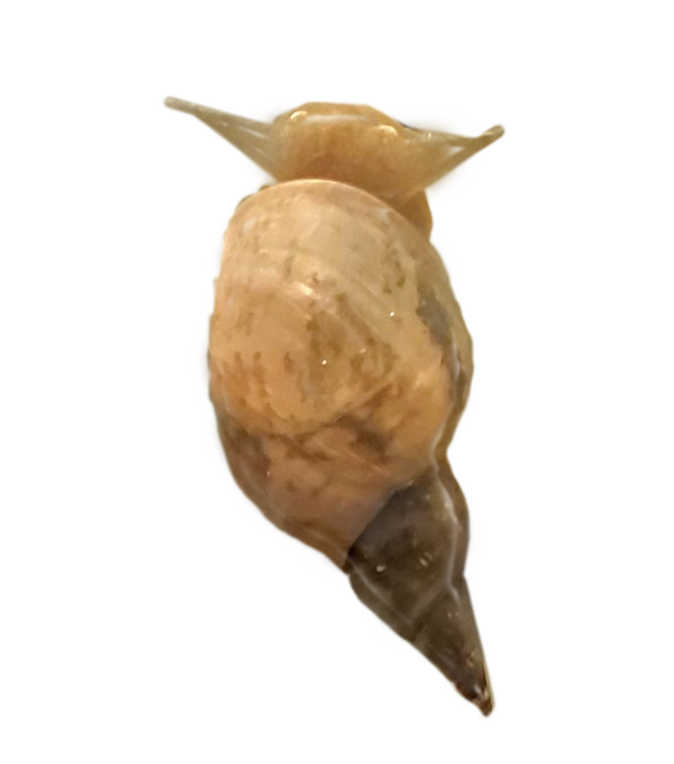
\includegraphics[width=0.7\linewidth]{img/intro/lymnaea.png} 
%	\caption{\textit{Lymnaea Stagnalis}}
%%	\label{fig:snail}
%\end{wrapfigure} 
in its CPG, including the three main interneurons conforming it \parencite{benjamin_snail_1989,benjamin_morphology_1979,rose_relationship_1979,brierley_behavioral_1997} and the modulatory neurons that influence the CPG activity such as SO and CGC neuron in the cerebral ganglia \parencite{rose_interneuronal_1981,mccrohan_patterns_1980,kemenes_multiple_2001}). Besides the buccal ganglia, other neurons in different ganglia are also well identified, with specific characteristics such as electrical coupling or dopamine containing neurons as in the Right Parietal Ganglia\parencite{benjamin_electrotonic_1986,winlow_multiple_1981}).

\begin{figure}[htb!]
	\begin{minipage}{0.35\textwidth}
	\centering
	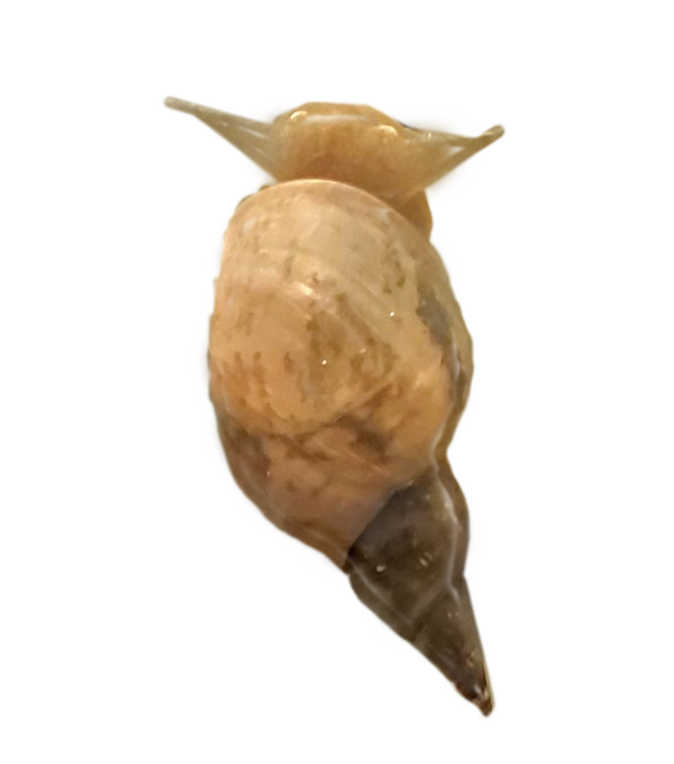
\includegraphics[width=\linewidth]{img/intro/lymnaea.png} 
	\caption{Imagen of \textit{Lymnaea Stagnalis}}
	\label{fig:snail}
	\end{minipage}
	\hfill
	\begin{minipage}{0.65\textwidth}
		\centering
		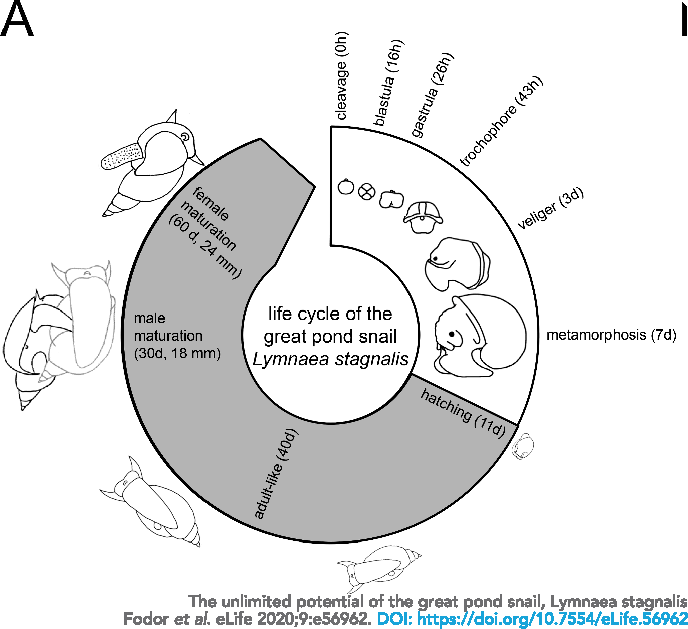
\includegraphics[width=\textwidth]{img/intro/lymnaea_life_cycle.pdf}
		\caption{Representation of \textit{L. stagnalis} life cycle. Figure 2A from \cite{fodor_unlimited_2020} (\href{http://creativecommons.org/licenses/by/4.0/}{Creative Commons license}).}
		\label{fig:lymnaea_life_cycle}
	\end{minipage}
\end{figure}

 From that point on, it has been key in other fields as host-parasite or genome editing. This last field is thanks to the short and well studied life-cycle in \textit{L. stagnalis} (see Fig. \ref{fig:lymnaea_life_cycle}), as well as the easiness to lab-bread them, without losing its main characteristics through generations \parencite{noland_observations_1946}. Recordings and analyses in this work are framed in the study of neural activity in it central nervous system (CNS). \textit{L. stagnalis} CNS is composed by 11 ganglia that conform the system: symmetrical pairs of buccal, pedal, cerebral, pleural and parietal, and a single visceral ganglia (see Sec. \ref{sec:lymnaea morphology}). We will focus specially in its feeding CPG, that by a distributed combination of motor- and inter-neurons allocated mainly in buccal and cerebral ganglia, produce a rhythmic pattern movement that allows feeding in three phases (protraction, rasp and swallow). Beyond this study of the CPG, we will work on the giant neurons located in the right parietal ganglia (RPG), enhancing the high-voltage (up to 80mV) and slow activity (30 to 100 ms per spike) to analyze in detail the action potential dynamics. 


\section{Neural stimulation}
\subsection{Stimulation techniques}

Neural stimulation have been an essential aspect in the study of neural dynamics, allowing the modulation of the neural system to explore, reproduce and alter its dynamics for their study. There are several techniques to produce the stimulation, we could classify them in chemical --using chemical components to block/enhance neural mechanisms--, electrical --injecting current in the cell membrane or nerves-- or optical --where neurons or circuits are stimulated though a illumination process. In this thesis,  we focus in the last two. In the electrical techniques, since the firsts applications of electrophysiology by \cite{neher_single-channel_1976} and the subsequent apparition of patch-clamp technique \cite{hamill_improved_1981}, many different techniques have been developed, for distinct systems. Voltage-clamp and patch clamping modified the paradigm in physiology and basic medicine in the study of the cell membrane dynamics with an exceptional detail that still today is heading ranges of precise recording and stimulation \parencite{hamill_improved_1981}. To Voltage-clamp followed variations such as dynamic-clamp, that enhances the electrophysiology possibilities by combining it with the possibilities of computing through a closed-loop protocol in real-time \parencite{nowotny_dynamic_2022}. This allows implementing specific algorithms to intervene the neural activity and test it to different approaches \parencite{chamorro_generalization_2012}. 
Regarding optical stimulation, a novel and widespread technique is opto-genetics, that by genetically modifying the animals, neurons are reactive to light and have had great achivements in the last decades using for both stimulation and exploration \parencite{chen_roles_2022}. Other example still understudy is near-infrared laser, a novel technique that will be explored in detail along this thesis. This technique have proven its potential for neuronal stimulation in different systems such as the hippocampus \parencite{liang_temperature-dependent_2009}, spinal ganglia in the cochlea \cite{goyal_acute_2012, barrett_pulsed_2018, brown_thermal_2020} and other systems \parencite{shapiro_infrared_2012, cayce_infrared_2014, begeng_activity_2022}.

%
%Apart from their possible subsequent aplication in clinical application, the use of these techniques for basis science is essential for a clear understanding of their implications, the biophysical mechanism they are able to alter and its safety range, and also for a wide understanding of the brain functioning.

\subsection{Neuromodulation and its need for clinical applications}


Beyond the necessity for neural stimulation in basic research to understand and explore the brain signaling and dynamics, there is a direct social impact for neural stimulation in clinical applications. In this context, Neuromodulation is an area of medicine involving many specialities that can be defined as "the science of how electrical, chemical and mechanical interventions can modulate distinct models of the nervous system function [and it is] inherently non-destructive, reversible, and adjustable" \parencite{krames_neuromodulation_2009}. This field is so important due to its possibilities in brain disorder treatments, for functional stimulation but also by the long-term modulation through neuronal plasticity. Neuromodulation can be classified, depending on the technology used for it, as invasive or non-invasive. Invasive technologies are those that require a direct interaction with the living system, which causes harm, e.g. including surgery. A well-known example of this type is deep-brain stimulation (DBS), this technique has been effectively used to treat movement disorders by electrically stimulating the brain at certain brain areas after implanting a device \parencite{limousin_long-term_2019, hariz_deep_2022}. In the case of non-invasive neuromodulation, we can find transcranial magnetic stimulation (TCM), that by electric fields stimulates certain areas of the brain, successful for example in the treatment of depression or obsessive compulsive disorder \parencite{valero-cabre_transcranial_2017, clarke_patients_2018}. Each type of technique has its own advantages, invasive techniques are usually more precise in space and time, whereas non-invasive techniques provide more flexibility and adaptability to different patients and the spreadness of the technique. In this context, the optical techniques discussed for stimulation in basic research have been rising in popularity also for clinical applications. 











